\begin{figure}
    \centering
        \vspace{-3mm}
    \begin{subfigure}{.45\textwidth}
        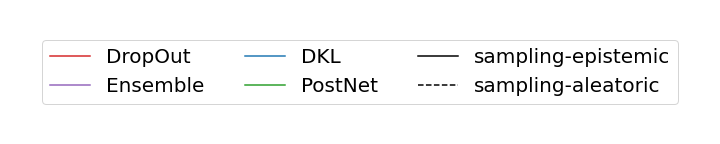
\includegraphics[width=\textwidth]{sections/011_icml2022/resources/sampling-legend.png}
    \end{subfigure}
    \vspace{-3mm}

    \begin{subfigure}{.24\textwidth}
        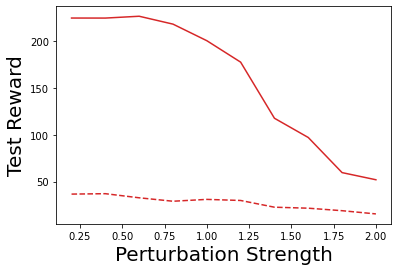
\includegraphics[width=\textwidth]{sections/011_icml2022/resources/action_shift-DropOut-CartPoleShift-v0-mean_reward_.png}
    \end{subfigure}
    \begin{subfigure}{.24\textwidth}
        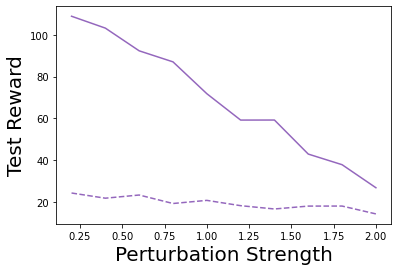
\includegraphics[width=\textwidth]{sections/011_icml2022/resources/action_shift-Ensemble-CartPoleShift-v0-mean_reward_.png}
    \end{subfigure}
    \begin{subfigure}{.24\textwidth}
        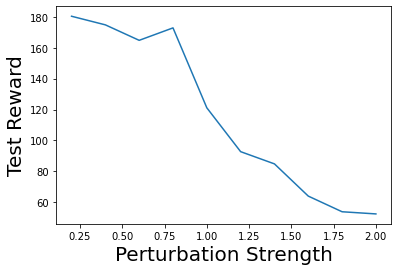
\includegraphics[width=\textwidth]{sections/011_icml2022/resources/action_shift-DKL-CartPoleShift-v0-mean_reward_.png}
    \end{subfigure}
    \begin{subfigure}{.24\textwidth}
        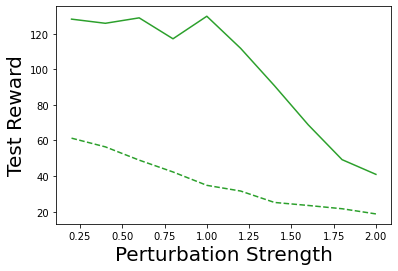
\includegraphics[width=\textwidth]{sections/011_icml2022/resources/action_shift-PostNet-CartPoleShift-v0-mean_reward_.png}
    \end{subfigure}
    
    \begin{subfigure}{.24\textwidth}
        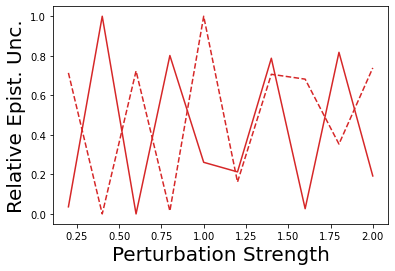
\includegraphics[width=\textwidth]{sections/011_icml2022/resources/action_shift-DropOut-CartPoleShift-v0-mean_epistemic_uncertainty_.png}
    \end{subfigure}
    \begin{subfigure}{.24\textwidth}
        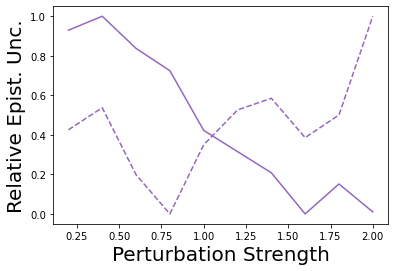
\includegraphics[width=\textwidth]{sections/011_icml2022/resources/action_shift-Ensemble-CartPoleShift-v0-mean_epistemic_uncertainty_.png}
    \end{subfigure}
    \begin{subfigure}{.24\textwidth}
        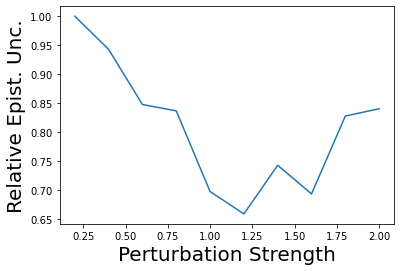
\includegraphics[width=\textwidth]{sections/011_icml2022/resources/action_shift-DKL-CartPoleShift-v0-mean_epistemic_uncertainty_.png}
    \end{subfigure}
    \begin{subfigure}{.24\textwidth}
        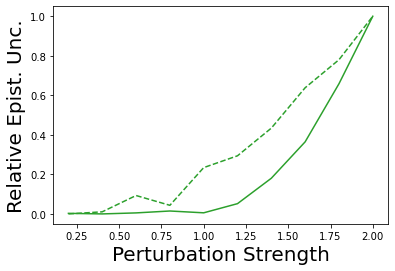
\includegraphics[width=\textwidth]{sections/011_icml2022/resources/action_shift-PostNet-CartPoleShift-v0-mean_epistemic_uncertainty_.png}
    \end{subfigure}
    \vspace{-3mm}
    \caption*{Action shifts}
    \vspace{2mm}
    
     \begin{subfigure}{.24\textwidth}
        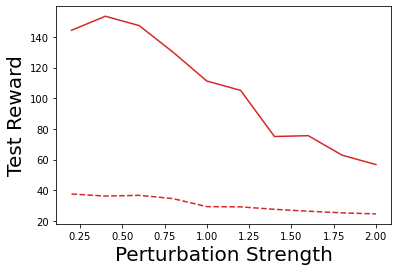
\includegraphics[width=\textwidth]{sections/011_icml2022/resources/state_shift-DropOut-CartPoleShift-v0-mean_reward_.png}
    \end{subfigure}
    \begin{subfigure}{.24\textwidth}
        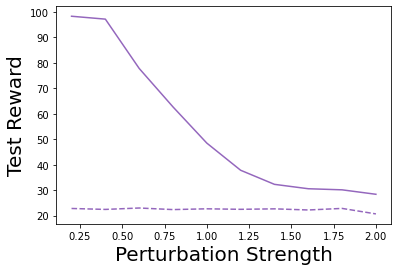
\includegraphics[width=\textwidth]{sections/011_icml2022/resources/state_shift-Ensemble-CartPoleShift-v0-mean_reward_.png}
    \end{subfigure}
    \begin{subfigure}{.24\textwidth}
        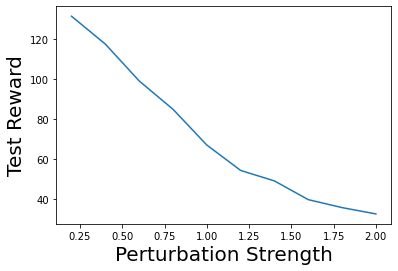
\includegraphics[width=\textwidth]{sections/011_icml2022/resources/state_shift-DKL-CartPoleShift-v0-mean_reward_.png}
    \end{subfigure}
    \begin{subfigure}{.24\textwidth}
        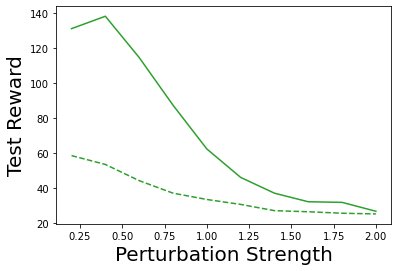
\includegraphics[width=\textwidth]{sections/011_icml2022/resources/state_shift-PostNet-CartPoleShift-v0-mean_reward_.png}
    \end{subfigure}
    
    \begin{subfigure}{.24\textwidth}
        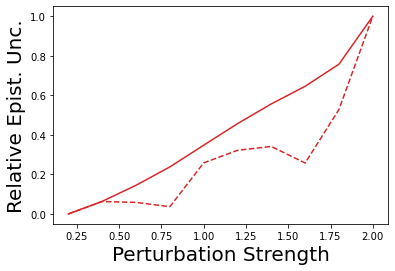
\includegraphics[width=\textwidth]{sections/011_icml2022/resources/state_shift-DropOut-CartPoleShift-v0-mean_epistemic_uncertainty_.png}
    \end{subfigure}
    \begin{subfigure}{.24\textwidth}
        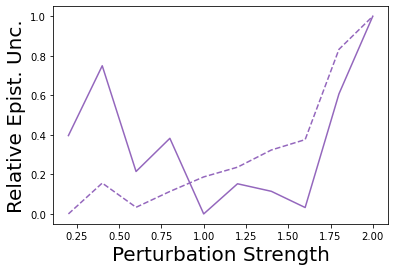
\includegraphics[width=\textwidth]{sections/011_icml2022/resources/state_shift-Ensemble-CartPoleShift-v0-mean_epistemic_uncertainty_.png}
    \end{subfigure}
    \begin{subfigure}{.24\textwidth}
        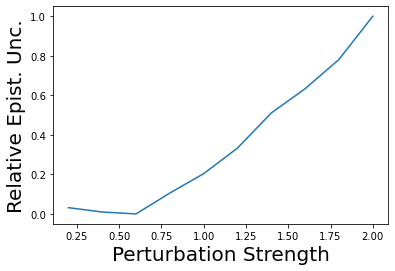
\includegraphics[width=\textwidth]{sections/011_icml2022/resources/state_shift-DKL-CartPoleShift-v0-mean_epistemic_uncertainty_.png}
    \end{subfigure}
    \begin{subfigure}{.24\textwidth}
        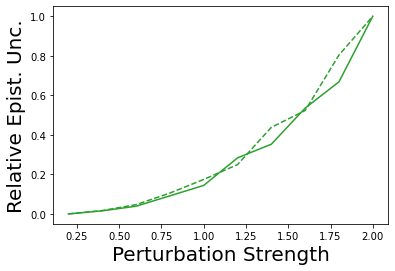
\includegraphics[width=\textwidth]{sections/011_icml2022/resources/state_shift-PostNet-CartPoleShift-v0-mean_epistemic_uncertainty_.png}
    \end{subfigure}
        \vspace{-3mm}
    \caption*{State shifts}
    \vspace{2mm}

    \begin{subfigure}{.24\textwidth}
        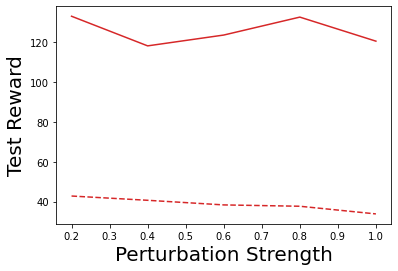
\includegraphics[width=\textwidth]{sections/011_icml2022/resources/transition_shift-DropOut-CartPoleShift-v0-mean_reward_.png}
    \end{subfigure}
    \begin{subfigure}{.24\textwidth}
        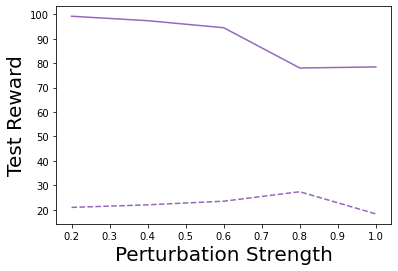
\includegraphics[width=\textwidth]{sections/011_icml2022/resources/transition_shift-Ensemble-CartPoleShift-v0-mean_reward_.png}
    \end{subfigure}
    \begin{subfigure}{.24\textwidth}
        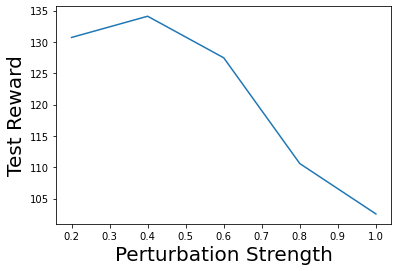
\includegraphics[width=\textwidth]{sections/011_icml2022/resources/transition_shift-DKL-CartPoleShift-v0-mean_reward_.png}
    \end{subfigure}
    \begin{subfigure}{.24\textwidth}
        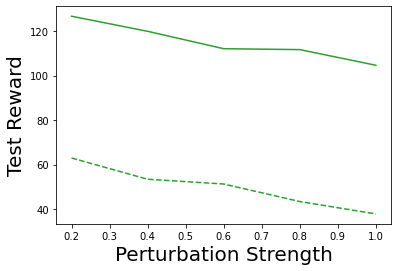
\includegraphics[width=\textwidth]{sections/011_icml2022/resources/transition_shift-PostNet-CartPoleShift-v0-mean_reward_.png}
    \end{subfigure}
    
    \begin{subfigure}{.24\textwidth}
        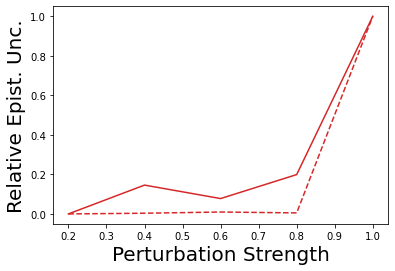
\includegraphics[width=\textwidth]{sections/011_icml2022/resources/transition_shift-DropOut-CartPoleShift-v0-mean_epistemic_uncertainty_.png}
    \end{subfigure}
    \begin{subfigure}{.24\textwidth}
        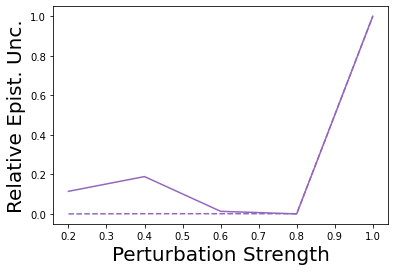
\includegraphics[width=\textwidth]{sections/011_icml2022/resources/transition_shift-Ensemble-CartPoleShift-v0-mean_epistemic_uncertainty_.png}
    \end{subfigure}
    \begin{subfigure}{.24\textwidth}
        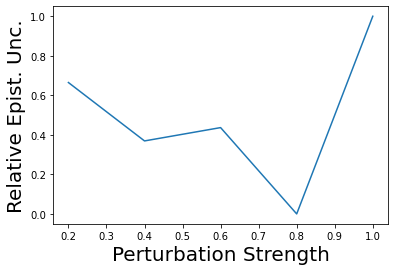
\includegraphics[width=\textwidth]{sections/011_icml2022/resources/transition_shift-DKL-CartPoleShift-v0-mean_epistemic_uncertainty_.png}
    \end{subfigure}
    \begin{subfigure}{.24\textwidth}
        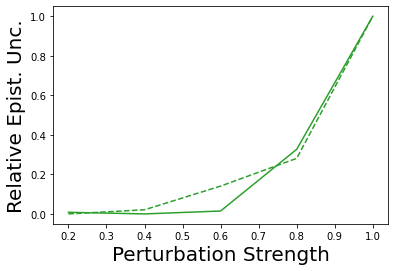
\includegraphics[width=\textwidth]{sections/011_icml2022/resources/transition_shift-PostNet-CartPoleShift-v0-mean_epistemic_uncertainty_.png}
    \end{subfigure}
    \vspace{-3mm}
    \caption*{Transition shifts}
    \vspace{2mm}

    \caption{Comparison of the testing performance and the epistemic uncertainty predictions on CartPole with perturbed actions, states, and transitions. The four uncertainty methods use the epsilon-greedy strategy at training time and the sampling-aleatoric or sampling-epistemic strategy at testing time. Ideally, an uncertainty aware model should maintain high reward while assigning higher epistemic uncertainty on more severe perturbations.}
    \label{fig:strategy-shift-testing-performance-cartpole}
        \vspace{-3mm}
\end{figure}